\documentclass[11pt]{article}
\usepackage[utf8]{inputenc} % Para caracteres en espa�ol
\usepackage{amsmath,amsthm,amsfonts,amssymb,amscd}
\usepackage{multirow,booktabs}
\usepackage[table]{xcolor}
\usepackage{fullpage}
\usepackage{lastpage}
\usepackage{enumitem}
\usepackage{multicol}
\usepackage{fancyhdr}
\usepackage{mathrsfs}
\usepackage{wrapfig}
\usepackage{setspace}
\usepackage{esvect}
\usepackage{calc}
\usepackage{multicol}
\usepackage{cancel}
\usepackage{graphicx}
\graphicspath{ {pictures/} }
\usepackage[retainorgcmds]{IEEEtrantools}
\usepackage[margin=3cm]{geometry}
\usepackage{amsmath}
\newlength{\tabcont}
\setlength{\parindent}{0.0in}
\setlength{\parskip}{0.05in}
\usepackage{empheq}
\usepackage{framed}
\usepackage[most]{tcolorbox}
\usepackage{xcolor}
\colorlet{shadecolor}{orange!15}
\parindent 0in
\parskip 12pt
\geometry{margin=1in, headsep=0.25in}
\theoremstyle{definition}
\newtheorem{defn}{Definition}
\newtheorem{reg}{Rule}
\newtheorem{exer}{Exercise}
\newtheorem{note}{Note}
\begin{document}
\setcounter{section}{0}

\thispagestyle{empty}

\begin{center}
{\LARGE \bf Section Template}\\
{\large AE435}\\
Spring 2018
\end{center}
\section{Section Title}
\subsection{Sub Section Title}
\subsubsection{Sub Sub Section Title}
\newpage
%%%%%%%%%%%%%%%%%%%%%%%%%%%%%%%%%%%%%%%%%%%%%%%%%%%%%%%%
%%%%%%%%%%%%%%                         BASIC TEMPLATES                                %%%%%%%%%%%%%%
%%%%%%%%%%%%%%%%%%%%%%%%%%%%%%%%%%%%%%%%%%%%%%%%%%%%%%%%
\section{Basic Templates}
% Basic Note Guides
\begin{note} \textbf{This is how you make numbered notes}\end{note}
\begin{exer} \textbf{This is how you make numbered exercises}\end{exer}
\begin{defn} \textbf{This is how you make numbered definitions}\end{defn}
\begin{reg} \textbf{This is how you make numbered rules}\end{reg}

%Shaded Equations + Explainer
\begin{shaded}
\textbf{Equation Name} \newline
\begin{equation*}
y = mx + b
\end{equation*}
Where:
\begin{equation*}
\begin{split}
variable1 &= \text{Description} \\
variable2 &= \text{Description} \\
\end{split}
\end{equation*}
\end{shaded}

%Insert Photo
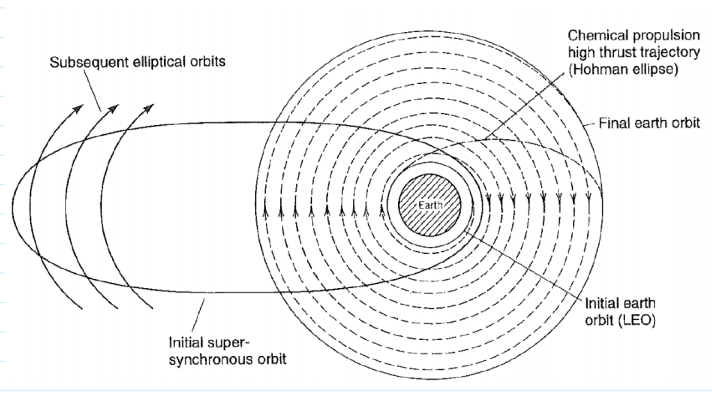
\includegraphics[scale=0.75]{1.png}

\end{document}